% called by main.tex
%
\chapter{Resultados}
\label{ch::capitulo7}

En este capítulo se presentan los datos resultantes de la investigación con el fin de observar el rendimiento de los diferentes modelos implementados y su comparación entre sí. 

En la \hyperref[figure11]{Figura 11}, se pueden observar para cada conjunto de datos evaluados, la mediana del MSE entre las distintas particiones de la evaluación \textit{Cross-Validation} para los modelos:

\begin{itemize}
    \item \texttt{RandomForestRegressor} (RF),
    \item \texttt{SharedKnowledgeRandomForestRegressor} (SK),
    \item \texttt{OOBRandomForestRegressor} (OOB),
    \item \texttt{IQRRandomForestRegressor} (IQR),
    \item \texttt{OOBPlusIQRRandomForestRegressor} (OOB+IQR),
    \item \texttt{PercentileTrimmingRandomForestRegressor} (PT) y
    \item \texttt{FirstSplitCombinerRandomForestRegressor} (FSC).
\end{itemize}

Con mayor detalle se presentan las mediciones para cada fold, dataset y modelo en el \hyperref[appendix8]{Apéndice 8}.

\begin{figure}[h]
\centering
    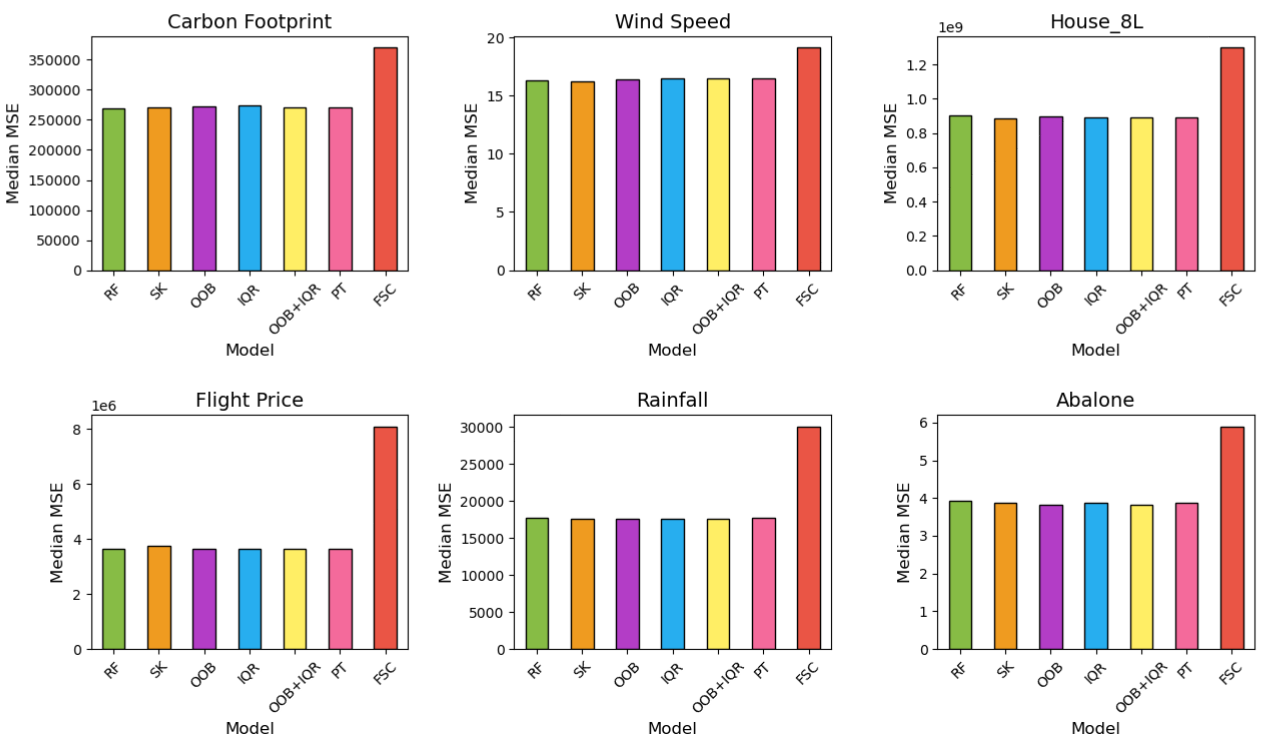
\includegraphics[width=1\textwidth]{figures/results/comparison_grid.png}
\caption{Mediana del MSE por modelo en cada dataset}
\end{figure}
\label{figure11}

\FloatBarrier

Por su parte, en la \hyperref[tab1]{Tabla 1} se presentan los resultados del test de hipótesis no paramétrico evaluado para comparar los modelos entre sí para cada uno de los conjuntos de datos seleccionados.

\begin{table}[h!]
\centering
\begin{tabular}{lcc}
\toprule
\textbf{Dataset} & \textbf{H-statistic} & \textbf{p-valor} \\
\midrule
Carbon Footprint & 20.4  & 0.002 \\
House 8L         & 13.5  & 0.035 \\
Wind Speed       & 7.86  & 0.25 \\
Rainfall         & 25.65 & 0.0003 \\
Flight Price     & 14.09 & 0.029 \\
Abalone          & 20.76 & 0.0020 \\
\bottomrule
\end{tabular}
\caption{Resultados del test de Kruskal-Wallis.}
\label{tab1}
\end{table}

\FloatBarrier

A su vez, para aquellos conjunto de datos en los cuáles se observó alguna diferencia significativa entre modelos, se muestran en las Tablas \hyperref[tab2]{2}, \hyperref[tab3]{3}, \hyperref[tab4]{4}, \hyperref[tab5]{5} y \hyperref[tab6]{6} los resultados del análisis post-hoc utilizando el test de Dunn.

\section*{}

\begin{longtable}{lccccccc}
\toprule
   & IQR     & PT     & OOB     & OOB+IQR     & FSC      & SK     & RF     \\
\midrule
IQR  & 1.0   & 1.0   & 1.0   & 1.0   & 0.015  & 1.0   & 1.0   \\
PT  & 1.0   & 1.0   & 1.0   & 1.0   & 0.014  & 1.0   & 1.0   \\
OOB  & 1.0   & 1.0   & 1.0   & 1.0   & 0.010  & 1.0   & 1.0   \\
OOB+IQR  & 1.0   & 1.0   & 1.0   & 1.0   & 0.012  & 1.0   & 1.0   \\
FSC  & 0.015 & 0.014 & 0.010 & 0.012 & 1.0    & 0.009 & 0.012 \\
SK  & 1.0   & 1.0   & 1.0   & 1.0   & 0.009  & 1.0   & 1.0   \\
RF  & 1.0   & 1.0   & 1.0   & 1.0   & 0.012  & 1.0   & 1.0   \\
\bottomrule
\caption{Carbon Footprint}
\end{longtable}
\label{tab2}

\begin{longtable}{lccccccc}
\toprule
   & IQR     & PT     & OOB     & OOB+IQR     & FSC      & SK     & RF     \\
\midrule
IQR  & 1.0   & 1.0   & 1.0   & 1.0   & 0.165  & 1.0   & 1.0    \\
PT  & 1.0   & 1.0   & 1.0   & 1.0   & 0.114  & 1.0   & 1.0    \\
OOB  & 1.0   & 1.0   & 1.0   & 1.0   & 0.100  & 1.0   & 1.0    \\
OOB+IQR  & 1.0   & 1.0   & 1.0   & 1.0   & 0.081  & 1.0   & 1.0    \\
FSC  & 0.165 & 0.114 & 0.100 & 0.081 & 1.0    & 0.068 & 0.159  \\
SK  & 1.0   & 1.0   & 1.0   & 1.0   & 0.068  & 1.0   & 1.0    \\
RF  & 1.0   & 1.0   & 1.0   & 1.0   & 0.159  & 1.0   & 1.0    \\
\bottomrule
\caption{House\_8L}
\end{longtable}
\label{tab3}

\begin{longtable}{lccccccc}
\toprule
   & IQR     & PT     & OOB     & OOB+IQR     & FSC      & SK     & RF     \\
\midrule
IQR  & 1.0   & 1.0   & 1.0   & 1.0   & 0.001  & 1.0   & 1.0    \\
PT  & 1.0   & 1.0   & 1.0   & 1.0   & 0.009  & 1.0   & 1.0    \\
OOB  & 1.0   & 1.0   & 1.0   & 1.0   & 0.002  & 1.0   & 1.0    \\
OOB+IQR  & 1.0   & 1.0   & 1.0   & 1.0   & 0.002  & 1.0   & 1.0    \\
FSC  & 0.001 & 0.009 & 0.002 & 0.002 & 1.0    & 0.001 & 0.003  \\
SK  & 1.0   & 1.0   & 1.0   & 1.0   & 0.001  & 1.0   & 1.0    \\
RF  & 1.0   & 1.0   & 1.0   & 1.0   & 0.003  & 1.0   & 1.0    \\
\bottomrule
\caption{Rainfall}
\end{longtable}
\label{tab4}

\begin{longtable}{lccccccc}
\toprule
   & IQR     & PT     & OOB     & OOB+IQR     & FSC      & SK     & RF     \\
\midrule
IQR  & 1.0   & 1.0   & 1.0   & 1.0   & 0.078  & 1.0   & 1.0    \\
PT  & 1.0   & 1.0   & 1.0   & 1.0   & 0.107  & 1.0   & 1.0    \\
OOB  & 1.0   & 1.0   & 1.0   & 1.0   & 0.070  & 1.0   & 1.0    \\
OOB+IQR  & 1.0   & 1.0   & 1.0   & 1.0   & 0.070  & 1.0   & 1.0    \\
FSC  & 0.078 & 0.107 & 0.070 & 0.070 & 1.0    & 0.213 & 0.070  \\
SK  & 1.0   & 1.0   & 1.0   & 1.0   & 0.213  & 1.0   & 1.0    \\
RF  & 1.0   & 1.0   & 1.0   & 1.0   & 0.070  & 1.0   & 1.0    \\
\bottomrule
\caption{Flight Price}
\end{longtable}
\label{tab5}

\begin{longtable}{lccccccc}
\toprule
   & IQR     & PT     & OOB     & OOB+IQR     & FSC      & SK     & RF     \\
\midrule
IQR  & 1.0   & 1.0   & 1.0   & 1.0   & 0.010  & 1.0   & 1.0    \\
PT  & 1.0   & 1.0   & 1.0   & 1.0   & 0.013  & 1.0   & 1.0    \\
OOB  & 1.0   & 1.0   & 1.0   & 1.0   & 0.006  & 1.0   & 1.0    \\
OOB+IQR  & 1.0   & 1.0   & 1.0   & 1.0   & 0.006  & 1.0   & 1.0    \\
FSC  & 0.010 & 0.013 & 0.006 & 0.006 & 1.0    & 0.016 & 0.024  \\
SK  & 1.0   & 1.0   & 1.0   & 1.0   & 0.016  & 1.0   & 1.0    \\
RF  & 1.0   & 1.0   & 1.0   & 1.0   & 0.024  & 1.0   & 1.0    \\
\bottomrule
\caption{Abalone}
\end{longtable}
\label{tab6}

Dada la diferencia particular del modelo \texttt{FirstSplitCombinerRandomForestRegressor}, de la cuál se desarrolla en \textit{\hyperref[ch::capitulo8]{Discusión}}, se re-evaluó el test de hipótesis quitando este modelo. Estos resultados se ven en la \hyperref[tab7]{Tabla 7}.

\begin{table}[h!]
\centering
\begin{tabular}{lcc}
\toprule
\textbf{Dataset} & \textbf{H-statistic} & \textbf{p-valor} \\
\midrule
Carbon Footprint & 0.04  & 0.99 \\
House 8L         & 0.18  & 0.99 \\
Wind Speed       & 0.13  & 0.99 \\
Rainfall         & 0.40 & 0.99 \\
Flight Price     & 0.25 & 0.99 \\
Abalone          & 0.30 & 0.99 \\
\bottomrule
\end{tabular}
\caption{Resultados del test de Kruskal-Wallis sin el modelo FSC.}
\label{tab7}
\end{table}
